\documentclass[mistar]{acmtrans2m}

%\usepackage[latin1]{inputenc}
\usepackage[T1]{fontenc}
\usepackage[portuguese]{babel}

\usepackage{graphicx}
\usepackage{listings}
\usepackage[usenames,dvipsnames]{color}
\usepackage[caption=false,font=footnotesize]{subfig}
\usepackage{pifont} % for \cross symbol newcommand
\usepackage{amsfonts}
\usepackage{url}

\definecolor{darkblue}{rgb}{0,0.1,0.5}

\lstdefinelanguage{codeTTN}
{
        basicstyle=\ttfamily\footnotesize,
        sensitive=true,
        showstringspaces=false,
        numberblanklines=true,
        showspaces=false,
        breaklines=true,
        showtabs=false,
		numbers=left,
		numberstyle=\footnotesize,
		xleftmargin=15pt,
}
\lstnewenvironment{code}{\lstset{language=codeTTN}}{}

\newtheorem{theorem}{Theorem}[section]
\newtheorem{conjecture}[theorem]{Conjecture}
\newtheorem{corollary}[theorem]{Corollary}
\newtheorem{proposition}[theorem]{Proposition}
\newtheorem{lemma}[theorem]{Lemma}
\newdef{definition}[theorem]{Definition}
\newdef{remark}[theorem]{Remark}

\newcommand{\checkK}{\color{ForestGreen}\checkmark}
\newcommand{\cross}{\color{red}\hspace{-3pt}\ding{55}}
\newcommand{\bigexclaim}{\color{Dandelion}$\bigtriangleup$\hspace{-5.6pt}!}
%Altere os seguintes dois par�metros.
%Os par�metros, normalmente nome do autor no primeiro e  t�tulo do artigo no segundo, sero inseridos nos cabe�alhos das p�ginas pares e �mpares respectivamente.
\markboth{Ulisses Ara�jo Costa}{Automatic Test Generation for Space}

%Nome do Artigo
\title{Automatic Test Generation for Space}

 %Autor, em mai�sculas, e institui��o, neste caso Universidade do Minho
\author{Ulisses Ara�jo Costa\\University of Minho}

\begin{abstract}
The European Space Agency (ESA) uses an engine to perform tests in the
Ground Segment infrastructure, specially the Operational Simulator.
This engine uses many different tools to ensure the development of
regression testing infrastructure and these tests perform black-box
testing to the C++ simulator implementation.
VST (Visionspace Technologies) is one of the companies that provides
these services to ESA and they need a tool to instead of writing
manually scripts to perform tests, it should try to automatically
infer tests from the existing C++ code.

%There are many approaches trying to tackle this problem and therefore
%many tools were developed.
%Automated Test Case Generation tools give support for creating test
%cases and at the same time ensure test case coverage methodically. The
%main goal of this tools is extract information from the program on how
%to generate executable test cases.
%Using manual written tests is tedious, time consuming and error-prone.
%Lots of functions/methods need full code coverage and this technique
%leaves to incomplete test suites and is hard to create tests that
%cover specific code paths potentially leaving many hidden bugs.
%Besides that, software is not a static artifact and is constantly
%evolving, so a test generation technique could be a more suitable
%mechanism in the development process.
\end{abstract}

\category{D.2.5}{Software Engineering}{Testing and Debugging}

\terms{Languages, Verification}

 %palavras chaves
\keywords{
Automatic Test Generation,
UML/OCL,
White-box testing,
Black-box testing
}

\begin{document}
\setcounter{page}{1}%Alterar "1" para a p�gina a ser indicada pela equipa do DI-RPD.

\begin{bottomstuff}
ucosta@visionspacetech.com
\end{bottomstuff}

\maketitle

\section{Introduction}\label{introd}
Since ever, every industry use testing methods to discover problems in early stages of development process to improve
the products quality and software industry is not an exception. Miller\cite{miller} describe the utility
of software testing as:

\begin{quotation}
The general aim of testing is to affirm the quality of software systems by systematically
exercising the software in carefully controlled circumstances.
\end{quotation}

In the most recent period of software history the integration of
software testing as an important step in the process of
software development opened up to the origin of \textit{xUnit}\cite{xunit}
tools and Agile software development.
Also, ESA started to use manual written tests as a part of their
software development processes.\\
Using  manual written tests is tedious, time consuming and error-prone.
Lots of functions/methods need full code coverage and this technique
leads to incomplete test suites;
as it is hard to create tests that cover specific code paths, many
hidden bugs can be left.
Many times a supervision leaded by the developer
is needed to assure that the right paths in the code are being tested,
specially regarding black-box testing.\\
Nowadays we start to observe a rapid increase in the automatic test
generation field.

\subsection{Goals}
This document reviews the most studied techniques
and the tools that implement them in order to choose the best set of
suitable techniques to incorporate in a automatic
testing generator to the Ground Segment infrastructure, specially the
Operational Simulator at ESA.\\
Two different techniques emerge for different purposes, Structural
Techniques and Functional Techniques,
known respectively as White-box testing and Black-box\cite{black} testing.
Functional testing is the most common at ESA, because of the
calculation complexity behind the Operational Simulators.\\
A briefly discussion will be presented regarding White-box testing vs. Black-box
testing and from there will be explained in more detail some automatic
generation techniques. Furthermore will be shown the potential of the described tools.

\subsection{White-box vs Black-box testing}
In White-box testing the tester needs to understand the internals of
the code to be able to write tests for it.
The goal of selecting test cases that test specific parts of the code
is to cause the execution of specific spots in the software, such as
statements, branches or
paths.
This technique consists in analyzing statically a program, by reading
the program code and using symbolic execution techniques to simulate
abstract program
executions in order to attempt to compute inputs to drive the program
along specific execution paths or branches, without ever executing the
program.\\
Control Flow based testing approach can be useful to analyze all the
possible paths in the code and write unit tests to cover multiple paths.
CFG (Control Flow Graph) of the program can be built,
test inputs can be generated to make any path execute regarding a given criterion:
Select all paths;
Select paths to achieve complete statement
coverage\cite{stt,Ntafos:1988:CST:630792.631017};
Select paths to achieve complete branch coverage\cite{Roper1994,stt};
or Select paths to achieve predicate
coverage\cite{stt,Ntafos:1988:CST:630792.631017}.

Data Flow Testing is designed into looking at the life cycle
(creation, usage and destruction) of a particular
piece of data and observe how it is used along the CFG, this ensures
that the number of paths are always finite\cite{dataflow}.\\

Opposite to White-box testing, Black-box testing is based on
functionality, so the tester observes a system based
on its functional contracts and writes the pairs of inputs and the
expected outputs.
This approach is used for unit testing of single methods/functions,
integration testing
of combinations of the methods/functions, or even final system testing.\\

This document is organized as follows.
In Section~\ref{testingapproaches} the important testing approaches in
use---Specification-based testing and Constraint-based generation---are briefly
revisited and, for each one,  the most relevant
tools are identified.
In Section~\ref{testingtools} some of the tools referred are
experimented in order to be compared.
Our proposal for a test generation system is introduced in
Section~\ref{proposal}.
The document is concluded in Section~\ref{Concl}.

\section{Testing Tools Approaches}\label{testingapproaches}
Here will be presented a study on the most recent tools that uses: Specification-based testing and
Constraint-based generation for the most used languages - C, JAVA and C\#.

% Specification Based Testing:
% http://cs.union.edu/~barrv/Testing/Labs/lab9.html
% Video:
% http://www.youtube.com/watch?v=caElFKbceP0
% Program Veri�cation - Automated Test Case Generation, Part I
% https://docs.google.com/viewer?a=v&q=cache:xNINgGyegt8J:www.cs.uiowa.edu/~tinelli/classes/181/Spring08/Notes/10-ATCG-1.pdf+automatic+testcase+generation+-gui+-uml+-web&hl=pt-PT&gl=pt&pid=bl&srcid=ADGEESg65_S-6rwRNXFWJZjChW3x1J4oIldqfY6feMxBYdluY2LkCivOB8fs19Wtg6z1fhTpvrOQYBiIIyUv_3aRnJS3rzZSBjtnuHvtz3fx48xdJW6Jfj66_YvsMcaInpcw3xmO8t0Z&sig=AHIEtbTkPm7QVWO3evlUquwqV8LT-PvtBA
% http://cs.gmu.edu/~offutt/rsrch/spec.html
% Practical Model-Based Testing: A Tools Approach
% http://www.cs.waikato.ac.nz/research/mbt/
% MODEL BASED TEST GENERATION TOOLS
% http://www.geocities.com/model_based_testing/
% http://www.agedis.de/documents/ModelBasedTestGenerationTools_cs.pdf
% Wikipedia
% http://en.wikipedia.org/wiki/Model-based_testing
% Microsoft Spec# model-based presentation (for dummies)
% https://docs.google.com/viewer?a=v&q=cache:PVdrO7s75ScJ:www.sasqag.org/pastmeetings/harryr.ppt+model+based+testing&hl=pt-PT&gl=pt&pid=bl&srcid=ADGEESjsdNheYbIWtyBYEfgNss2mRQuVcH0Kh8nejgxYwFMSSoPDuEgtZbxdchxcNXENujrMXaIeDr4Q17lpB1Kk8073iuk76o6G66sppEYAq8wGbUKnNtbOx4eHlT_P2boklZ_DwiO&sig=AHIEtbTECVDePxriKz0fNYbhSo56Ktgvww
%Predicates as specifications (Alloy is related to OCL (Object Constraint Language) for UML)
\subsection{Specification-based Generation Testing}
Specification Based Testing also known as Model Based Testing refers to the process of testing a program based on what its specification or model says its behavior should be.
In particular, can be generated test cases based on the specification of the program's behavior, without seeing an implementation of the program. So this clearly a
way of Black-box testing.\\
With this technique the testing phase and development phase can be started in parallel, don't need the implementation
to start the development of test cases. The only thing needed is the functional contracts and/or oracles for each function/method.\\
Since the 90's there have been some effort into using specifications to try to generate test cases such as Z specifications
\cite{Horcher95improvingsoftware,Stocks:1996:FST:239916.239918}, UML statecharts\cite{Offutt:1999:GTU:1767297.1767341},VDM\cite{Aichernig99automatedblack-box}
or ADL specifications\cite{Sankar94specifyingand}.
These specifications typically do not consider structurally complex inputs and these tools do not generate junit test cases.
Nowadays there are some tools out there that can perform Specification-based Testing approach:

\begin{description}
\item[Conformiq] is a commercial Tool Suite that generates
human-readable test plans and executable test scripts from Java code, state charts and UML\footnote{See more at: \url{http://www.conformiq.com/products.php}}.
\item[MaTeLo] stands for Markov Test Logic and is a commercial tool
that generates test sequences from a collection of states, transitions, classes of equivalence, types, sequences, global variables and test oracles
using their user interface\footnote{See more at: \url{http://www.all4tec.net/index.php/All4tec/matelo-product.html}}.
\item[Smartesting CertifyIt] is a commercial tool that generates test cases from a functional model, as UML\footnote{See more at: \url{http://www.smartesting.com/index.php/cms/en/product/certify-it}}.
\item[T-Vec] is a commercial tool that generates test cases from modeling tools available from T-VEC or third-party vendors\footnote{See more at: \url{http://www.t-vec.com/}}.
\item[Rational Tau] is an IBM commercial tool that provides automated error checking, rules-based model checking, and a model-based explorer using
UML\footnote{See more at: \url{http://www-01.ibm.com/software/awdtools/tau/}}.
\end{description}
The most relevant ones or the more recent open-source ones will be discussed.

\subsubsection{Korat}
Korat\cite{Boyapati02korat:automated} is a mature framework for automated testing structurally complex inputs of JAVA programs.
Given a formal specification for a method, Korat\footnote{See more at: \url{http://korat.sourceforge.net/}} uses the method precondition
to automatically generate all (nonisomorphic) test cases up to a given small size.
Korat then executes the method on each test case, and uses the method postcondition as a test oracle to check the correctness of each output.\\
To be able to generate test cases for a method, Korat uses a predicate and a bound on the size of its inputs,
Korat generates all (nonisomorphic) inputs for which the predicate returns $true$.
Korat generates all the possible input spaces regarding the predicate and monitor the predicate's executions to be able to prune large portions of the search space.\\
\indent The writing of a predicate is done using JAVA language and in most cases can be written the first thing that cames to programmer's head to restrict the input space.
But for more complex structures it is better to understand how the matching algorithm work to be able to write a fast verifiable predicate.\\
Unfortunately the test derivation tool using Korat (that also uses JML) is not available to the public.

\subsection{Constraint-based Generation Testing}
Constraint Based Testing\cite{DeMillo91constraint-basedautomatic} can be used to select test cases satisfying specific constraints by
solving a set of constraints over a set of variables. The system is described using constraints and these can be solved by SAT solvers.\\
Constraint programming can be combined with symbolic execution, regarding this approach a program is executed symbolically,
collecting data constraints over different paths in the CFG, and then solving the constraints and producing test cases from there.
This is clearly a White-box testing approach.
There are some tools out there, like:

\begin{description}
\item[Euclide] for verifying safety properties over C code using ACSL annotations, CPBPV for program verification.
\item[OSMOSE] a tool that uses concolic execution and path-based techniques over machine code.
\item[GATeL] for Lustre language to generate test sequences\footnote{See more at: \url{http://www-list.cea.fr/labos/gb/LSL/test/gatel/index.html}}.
\end{description}

Here two tools will be explained, one proprietary and other academic.

\subsubsection{Pex} Pex\cite{Tillmann:2008:PWB:1792786.1792798} is an automatic white-box test generation tool for .NET. Starting from a
method that takes parameters, Pex performs path-bounded model-checking
by repeatedly executing the program and solving constraint systems to obtain inputs that will steer the program along different execution paths.
This uses the idea of dynamic symbolic execution\cite{Tillmann06unittests}. Pex uses the theorem prover and
constraint solver Z3\footnote{See more at: \url{http://research.microsoft.com/en-us/um/redmond/projects/z3/}} to reason about the feasibility of execution paths, and
to obtain ground models for constraint systems.\\
Pex came with Moles that helps to generate unit tests. This tools together are able to understand the input (by analyzing branches in the code:
declarations, all exceptions throws operations, if statements, asserts and .net Contracts). With this information Pex uses Z3 constraint solver to
produce new test inputs which exercise diferent program behavior.\\
The result is an automatically generated small test suite which often achieves high code coverage.\\
Pex can be used in a project, class or method (which make it a very helpful and versatile tool). After the analysis process the "Pex Explorarion Results" shows
the $input \times output$ pairs selected for each test case for the method, here it also shows the percentage of the test coverage.

\subsubsection{PathCrawler} This is an academic tool based on dynamic and statical analysis\cite{Williams05pathcrawler:automatic}, 
it uses constraint logic programming to generate the Test-cases. PathCrawler\footnote{See more at: \url{http://www-list.cea.fr/labos/gb/LSL/test/pathcrawler/index.html}} executes an instrumented function for each function under test
with the generated inputs, it preserves this information to not cover the same path.\\
This tool supports assertions in any point in the code and pre-conditions regarding the input values.

\section{Using the tools}\label{testingtools}
After introducing the theory and the techniques that support each tool will be demonstrated some of the tools in action, regarding small but illustrative examples
on how each tool can help us find good test cases.\\

\subsection{PathCrawler}
Concerning the first case will be used a simple example based on a function that uses a multiplication, creating a simple branche on the code.
\begin{code}
typedef struct s {
    int x;
    int y;
}Point;

int Multiply(Point p) {
    if(p.x * p.y == 42) return 1;
    else return 0;
}
\end{code}
Pointers were tried instead of coping the structure as a parameter to $Multiply$ function, but PathCrawler was not able to run.

Nevertheless, PathCrawler was able to give a full coverage for this simple function as you can see in Table \ref{tab:mul}.

\begin{table}[!ht]
\renewcommand{\arraystretch}{1.3}
\setlength{\tabcolsep}{10pt}
\caption{Output Table for $Multiply$ function using PathCrawler}
\label{tab:mul}
\centering
\noindent \begin{tabular}{|c|c|c|}\hline
Result & p & return value\\\hline
\checkK & Point\{x=1,y=42\} & 1 \\\hline
\checkK & Point\{x=177407,y=109471\} & 0 \\\hline
\end{tabular}
\end{table}

Regarding our second example a function that performs a binary search in order to find if a number is in a given range (between two bounds).

\begin{code}
int BSearch(int x, int n) {
    return BinarySearch(x, 0, n); 
}
	
int BinarySearch(int x, int lo, int hi) {
    while (lo < hi) {
        int mid = (lo+hi)/2;
        pathcrawler_assert(mid >= lo && mid < hi);
        if (x < mid) { hi = mid; }
		else { lo = mid+1; }
    }
    return lo; 
}
\end{code}
A function that PathCrawler give to us has been used: $pathcrawler\_assert$, this function can be used at any location in the
program under test, and will force PathCrawler to generate test cases to cover both the case where its argument is true and the case where it is is false.
This feature may be seen as another way to write an oracle.\\
The results were interesting: 31 covered paths and 44 infeasible paths and the test as interrupted by PathCrawler,
because PathCrawler reach the maximal test session time (the user can increase this number, but for this example is left the default value).\\
A further analysis of the results demonstrated that 28 out of the 44 infeasible paths discovered appeared when PathCrawler tried to
do the assertion in line 8. Was not written any pre-condition, so PathCrawler does not know that this is a pre-condition
for $BinarySearch$ function:  $lo\leq~x<hi$. In Table \ref{tab:bsearch} is shown some of the test inputs generated for this example.

\begin{table}[!ht]
\renewcommand{\arraystretch}{1.3}
\caption{Output Table for $BSearch$ function using PathCrawler}
\label{tab:bsearch}
\centering
\noindent \begin{tabular}{|c|c|c|c|}\hline
Result & x & n & return value \\\hline
\checkK & -189424 & -140714 & 0 \\\hline
\checkK & 157819 & 0 & 0 \\\hline
\checkK & 1 & 1610612736 & 2 \\\hline
\checkK & 2 & 805306368 & 3 \\\hline
\checkK & 11 & 1610612736 & 12 \\\hline
\end{tabular}
\end{table}

PathCrawler was tried with the following function that calculates the year of the $n^{th}$ day after 1980-01-01.

\begin{code}
int IsLeapYear(int year) {
  return (year % 4 == 0) && ((year % 100 != 0) || (year % 400 == 0));
}
int FromDayToYear(int day) {
  int year = 1980;

  while (day > 365) {
    if (IsLeapYear(year)) {
      if (day > 366) {
        day -= 366;
        year += 1;
      }
    } else {
      day -= 365;
      year += 1;
    }
  }
  return year;
}
\end{code}

The result was unexpectedly $unknown$. PathCrawler was unable to trace even one path in our code, the number of $k$-path's could
be increased but with no success for this example.

\subsection{Pex}
Regarding Pex is used the same examples showed previously adapted to C\# language.
Because C\# is a more expressive language than C our examples will be improved with some other OO and C\# specific features like Exceptions and Debug.Assert calls.
In fact Pex can also support a lot more features that are present in C\# language like .NET Contracts and many more.\\
This is the simple implementation of a 2D $Point$ class that has been created to have special behavior, under a certain condition
$x \times y \equiv 42$ it is supposed to throw an exception.

\begin{code}
public class Point {
  public readonly int X, Y;
  public Point(int x, int y) { X = x; Y = y; }
}

public class Multiply {
  public static void multiply(Point p) {
    if (p.X * p.Y == 42)
        throw new Exception("hidden bug!");
  }
}
\end{code}

So, as was described earlier, Pex will try to generate such input as it is possible (in a given amount of time) to traverse all the paths inside the code.
The output table can be seen in Table \ref{tab:point}, with the inputs and outputs that Pex found to ensure a full coverage of the code.

\begin{table}[!ht]
\renewcommand{\arraystretch}{1.3}
\setlength{\tabcolsep}{1pt}
\caption{Output Table for $multiply$ method using Pex}
\label{tab:point}
\centering
\noindent \begin{tabular}{|c|c|c|c|}\hline
Result & p & Output/Exception & Error Message\\\hline
 &  &  & Object ref. not set \\
\cross & null  & NullReferenceException & to an instance \\
 &  &  & of an object.\\\hline
\checkK & new Point\{X=0,Y=0\} & &\\\hline
\cross & new Point\{X=3,Y=14\} & Exception & hidden bug!\\\hline
\end{tabular}
\end{table}

Pex was successful to reach the $Exception$ path inside the code. Of course this is not always possible, since sometimes the functions inside
the $if$ statement does not have inverse function.\\

Pex can also be very helpful checking assertions and contracts in .net code. A binary search algorithm was written and an assertion was also written in
the middle of our code.

\begin{code}
public class Program {
  public static int BSearch(int x, int n) {
    return BinarySearch(x, 0, n);
  }
  static int BinarySearch(int x, int lo, int hi) {
    while (lo < hi) {
      int mid = (lo+hi)/2;
      Debug.Assert(mid >= lo && mid < hi);
      if (x < mid) { hi = mid; } else { lo = mid+1; }
    }
    return lo;
  }
}
\end{code}

Pex was able to generate an input that could not pass in the assertion inerted in our code, as can be seen in Table \ref{tab:binary}.

\begin{table}[!ht]
\renewcommand{\arraystretch}{1.3}
\setlength{\tabcolsep}{1pt}
\caption{Output Table for $BSearch$ method using Pex}
\label{tab:binary}
\centering
\noindent \begin{tabular}{|c|c|c|c|c|}\hline
Result & x & n & result & Output/Exception \\\hline
\checkK & 0 & 0 & 0      & \\\hline
\checkK & 0 & 1 & 1      & \\\hline
\checkK & 0 & 3 & 1      & \\\hline
\cross & 1073741888 & 1719676992 & & TraceAssertionException \\\hline
\checkK & 1 & 6 & 2      & \\\hline
\checkK & 50 & 96 & 51      &\\\hline
\end{tabular}
\end{table}

\subsection{Korat}
Like was explained before, Korat generates a graphical representation of the structure instances that validates the property $repOK$. This property was written using JAVA code.\\
In order to test the freelly available version of Korat, a Doubly Linked List structure was created in JAVA.

\begin{code}
public class LinkedList<T> {
  public static class LinkedListElement<T> {
    public T Data;
    public LinkedListElement<T> Prev;
    public LinkedListElement<T> Next;
  }
  private LinkedListElement<T> Head;
  private LinkedListElement<T> Tail;
  private int size; 
}
\end{code}

\def\t#1#2#3#4{\langle#1 \ #2 : #3 \ : #4 \ \rangle}
\def\d#1#2#3{\langle#1 \ #2 :: #3 \ \rangle}
\newcommand{\subseteqL}{\mathbin{\subseteq\mkern-4mu\subseteq}}
\newcommand{\inL}{\mathbin{\in\mkern-4mu\in}}

Now the $repOK$ predicate method must be defined.
This predicate method will check that the tree doesn't have any cycles and that the number of nodes traversed from root matches the value of the field size.
First was defined the properties about this data structure. The most relevant ones are property \ref{eq:linked} in Figure \ref{fig:formulae} that
ensures the structure and property \ref{eq:uniq} that ensures our doubly linked list does not have repeated elements.\\
Consider $e,e_1,e_2 \in LinkedListElement$ and $i$ the index function: $i : LinkedListElement \rightarrow int$, that receives an element of $LinkedList$ and
returns the position of that element in the structure. Consider also three new functions:
\begin{enumerate}
\item $Head(l)$ being $l$ of type $LinkedList$ and meaning in Java code $l.Head$.
\item $Tail(l)$ being $l$ of type $LinkedList$ and meaning in Java code $l.Tail$.
\item $size(l)$ being $l$ of type $LinkedList$ and meaning in Java code $l.size$.
\end{enumerate}

As a matter of avoiding verbosity two symbols were defined:
\begin{enumerate}
\item $a \inL l$ being $a$ of type $LinkedListElement$ and meaning that $a$ is an element of the $LinkedList$ $l$.
\item $\{a,\ldots,z\} \subseteqL l$ meaning $a \inL l \wedge \ldots \wedge z \inL l$.
\end{enumerate}

\begin{figure*}[!Ht]
\begin{eqnarray}
\t \forall {l} {l \in LinkedList} {Head(l) \equiv null \vee Tail(l) \equiv null \Leftrightarrow size(l) \equiv 0}\\
\t \forall {l} {l \in LinkedList} {Tail(l).Next \equiv null}\\
\t \forall {l} {l \in LinkedList} {Head(l).Prev \equiv null}\\
\t \forall {l} {l \in LinkedList} {size(l) \equiv 1 \Leftrightarrow Head(l) \equiv Tail(l)}\\
\t \forall {l} {l \in LinkedList} {\t \forall {e_1,e_2} {\{e_1,e_2\} \subseteqL l} {\t \exists {e} {e \inL l} {e_1.Next \equiv e \wedge e_2.Prev \equiv e}}\label{eq:linked}}\\
\t \forall {l} {l \in LinkedList} {\t \forall {e_1,e_2} {\{e_1,e_2\} \subseteqL l} {e_1 \equiv e_2 \Rightarrow i(e_1) \equiv i(e_2)}\label{eq:uniq}}
\end{eqnarray}
\caption{Invariants for class $LinkedList$}
\label{fig:formulae}
\end{figure*}

The properties in Fig. \ref{fig:formulae} were taken and used to restrict the generation of structures using Java. So the $repOK$ method that receives
a $LinkedList$ structure and returns $Bool$ whenever this structure follows the invariants in \ref{fig:formulae} was defined.
Using this specification Korat generated the 2 structures showed in Figure \ref{fig:insts}. In Figure \ref{fig:inst1} with $2$ elements
and in Figure \ref{fig:inst2} an instance with $5$ elements.

\begin{figure}[!ht]
\centerline{
\subfloat[Instance with $2$ elements for $LinkedList$]{
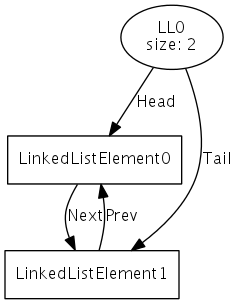
\includegraphics[width=.3\textwidth]{img/ll1}
\label{fig:inst1}
}
\hfil
\subfloat[Instance with $5$ elements for $LinkedList$]{
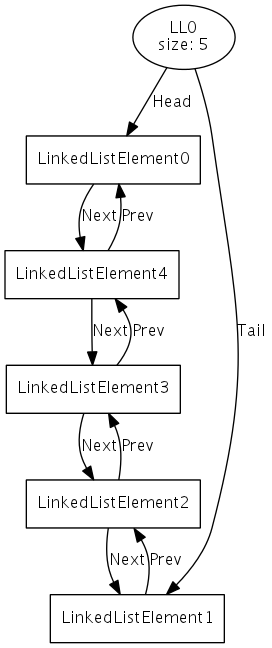
\includegraphics[width=.3\textwidth]{img/ll2}
\label{fig:inst2}}}
\caption{Examples of generated instances from Korat for $LinkedList$ class.}
\label{fig:insts}
\end{figure}

\subsection{Summary}
Was found that PathCrawler and Pex have different approaches regarding testcase generation. PathCrawler seems to be a very efficient tool to discover multiple
infeasible paths in C code, because it uses a mix between static and dynamic analysis, when it finds a suitable input for a function it tries to execute
collecting all the executed paths in the code.
Pex on the other side just uses static execution and it is very efficient discovering all the feasible paths in C\# methods. Pex was also used
to perform testcase generation in C\# classes, but the generated instances are too simple to perform more interesting tests. The $LinkedList$ class was written
in C\# with many management methods implemented (Add, Remove, Find,\ldots). Pex generated very simple $LinkedList$'s structures to perform automatic test generation
for each implemented method. The problem is that the generated structures does not meet the properties about Doubly Linked Lists as you can see in Figure \ref{fig:pexG}.
\\
Regarding Korat, this is The tool to generate complex data structures. The freely available part of Korat show potential in expressing rules to hedge
the automatic generation of data structures.
\begin{figure}[!ht]
\centerline{
\subfloat[Example of Pex generated $LinkedList$ instance to test $Remove$ method]{
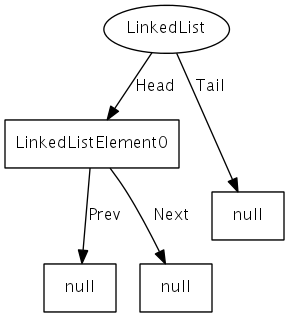
\includegraphics[width=.3\textwidth]{img/pex1}
\label{fig:pexinst1}
}
\hfil
\subfloat[Example of Pex generated $LinkedList$ instance to test $Find$ method]{
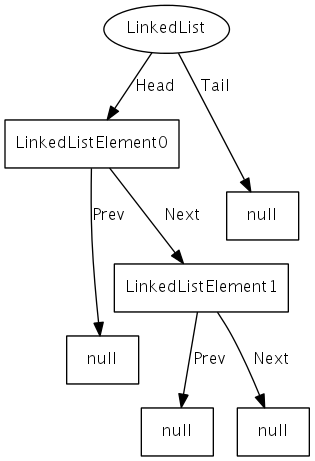
\includegraphics[width=.3\textwidth]{img/pex2}
\label{fig:pexinst2}}}
\caption{Examples of generated instances from Pex for $LinkedList$ class.}
\label{fig:pexG}
\end{figure}

\section{Generate Tests from Code+OCL}\label{proposal}
Since the Operational Simulator code is not familiar to us, was decided to start solving this problem by inferring the UML+OCL from the existing code
to be able to work on a more abstract level rather than the implementation. Our idea is from the generated OCL extract tests using the Partition Analysis described
in \cite{Benattou02generatingtest} and at the same time generate tests directly from the code, using static analysis methods - symbolic execution to complement
the specification-based generation from OCL. The main goal is to extract as many tests as possible from a model prospective and from the implementation prospective
to be able to feed a feedback loop\cite{Xie03mutuallyenhancing} generation testing framework with two tests prospectives: functional and structural and from there
be able to get a more refined set of tests.\\
A mixture between the symbolic execution from Pex and use the complex data generation from Korat will be developed
to be able to generate a more interesting inputs for the methods under testing.

\section{Conclusion}\label{Concl}
Pex has proved to be a very powerful tool trying to
give full coverage. Which was bit a disappointment was the lack of generation of calling methods sequence. With Microsoft's SpecExplorer we can already
manually call sequences of methods, maybe a combination of this feature with Pex would make Pex a perfect all-in-one testing tool regarding .NET automatic testing tools.\\
Regarding Korat, the expected step is just to write the invariants for a class instead of the $repOK$ method, or maybe infer these invariants 
from the existing code. Writing the $repOK$ method for very complex data structures requires for some previous experience with Korat, but we think
this is not a weakness, since it quickly gets used to write the $repOK$ method in Korat. The only problem is that right now we can not fully automate the process
without human help.\\
\indent Regarding the studied tools and thinking about a full automated test generation tool, a mix between Pex to ensure the maximum possible coverage, 
Korat to generate all the valid data structures and an automatic tool to generate calls to methods combinations would be the perfect tool.
With this document the first milestone is finished regarding the study of the state-of-the-art methods and some tools that
implement them. We have discussed some of the tested tools and present a mixture between some of them to be able to generate a more suitable
set of tests for each method/class. In the end is presented a brief idea on a Code+OCL method to infer tests from, based on some of the studied methods.\\
\indent Concerning the OCL inference from code, the solution is not yet done and work will be done on a tool that will be able to do it.
Is already known that is possible to infer pre-post-conditions\cite{moy} and interesting safety conditions using Frama-C.\\
%Bibliografia
\bibliography{mei-ptr-ulisses}%substituir o par�metro "bibtext" pelo nome do ficheiro (sem extens�o) que cont�m a bibliografia BibTex
\bibliographystyle{acmtrans}


\begin{received}
\end{received}
\end{document}

